% Created 2023-12-14 Thu 10:01
% Intended LaTeX compiler: pdflatex
\documentclass[presentation]{beamer}
\usepackage[utf8]{inputenc}
\usepackage[T1]{fontenc}
\usepackage{graphicx}
\usepackage{longtable}
\usepackage{wrapfig}
\usepackage{rotating}
\usepackage[normalem]{ulem}
\usepackage{amsmath}
\usepackage{amssymb}
\usepackage{capt-of}
\usepackage{hyperref}
\usepackage{listings}
\usepackage{tikz}
\usepackage{pgf}
\usetikzlibrary{positioning}
\setbeamercolor{title}{bg=white}
\setbeamercolor{frametitle}{bg=white}
\usetheme{default}
\usecolortheme{seahorse}
\author{Oskar Haukebøe}
\date{\today}
\title{Detection of shared network bottleneck using passive WiFi traffic analysis}
\hypersetup{
 pdfauthor={Oskar Haukebøe},
 pdftitle={Detection of shared network bottleneck using passive WiFi traffic analysis},
 pdfkeywords={},
 pdfsubject={},
 pdfcreator={Emacs 29.0.91 (Org mode 9.7-pre)}, 
 pdflang={English}}
\usepackage{calc}
\newlength{\cslhangindent}
\setlength{\cslhangindent}{1.5em}
\newlength{\csllabelsep}
\setlength{\csllabelsep}{0.6em}
\newlength{\csllabelwidth}
\setlength{\csllabelwidth}{0.45em * 0}
\newenvironment{cslbibliography}[2] % 1st arg. is hanging-indent, 2nd entry spacing.
 {% By default, paragraphs are not indented.
  \setlength{\parindent}{0pt}
  % Hanging indent is turned on when first argument is 1.
  \ifodd #1
  \let\oldpar\par
  \def\par{\hangindent=\cslhangindent\oldpar}
  \fi
  % Set entry spacing based on the second argument.
  \setlength{\parskip}{\parskip +  #2\baselineskip}
 }%
 {}
\newcommand{\cslblock}[1]{#1\hfill\break}
\newcommand{\cslleftmargin}[1]{\parbox[t]{\csllabelsep + \csllabelwidth}{#1}}
\newcommand{\cslrightinline}[1]
  {\parbox[t]{\linewidth - \csllabelsep - \csllabelwidth}{#1}\break}
\newcommand{\cslindent}[1]{\hspace{\cslhangindent}#1}
\newcommand{\cslbibitem}[2]
  {\leavevmode\vadjust pre{\hypertarget{citeproc_bib_item_#1}{}}#2}
\makeatletter
\newcommand{\cslcitation}[2]
 {\protect\hyper@linkstart{cite}{citeproc_bib_item_#1}#2\hyper@linkend}
\makeatother\begin{document}

\maketitle

\begin{frame}[label={sec:orgc0699d8}]{NETHINT}
\begin{columns}
\begin{column}{0.48\columnwidth}
\begin{itemize}[<+->]
\item Part of earlier master thesis
\item Determine whether network congestion is located on local WiFi or not
\item Know whether you can blame your family for slow internet
\item Only uses passive measurements
\end{itemize}
\end{column}
\begin{column}{0.7\columnwidth}
\begin{center}
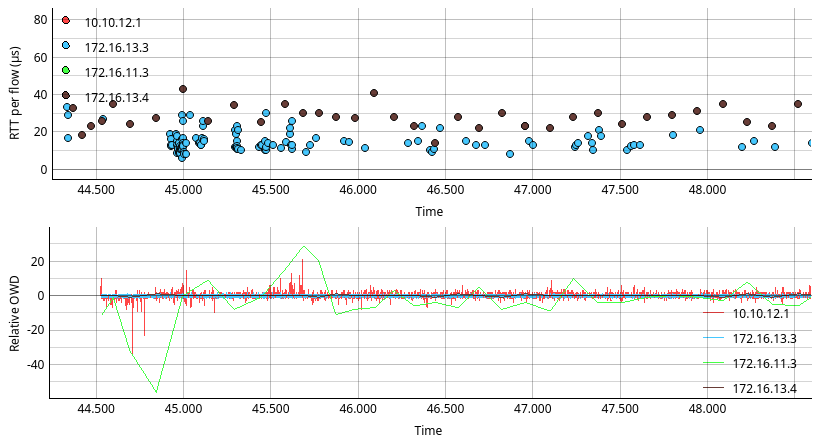
\includegraphics[width=.9\linewidth]{figures/nethint.png}
\end{center}
\end{column}
\end{columns}
\end{frame}
\begin{frame}[label={sec:org0419901}]{TEACUP}
\pause

\begin{center}
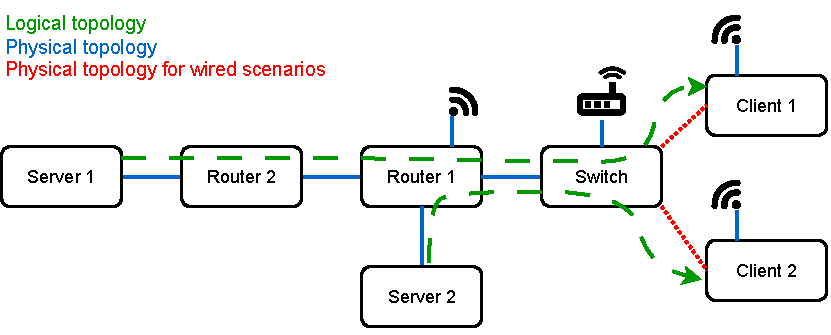
\includegraphics[width=.9\linewidth]{figures/topology-wireless.drawio-1.pdf}
\end{center}
\end{frame}
\begin{frame}[label={sec:org8cbd992}]{Traffic generation}
\begin{tikzpicture}[remember picture, overlay]
\node[below left] at (current page.north east)
{
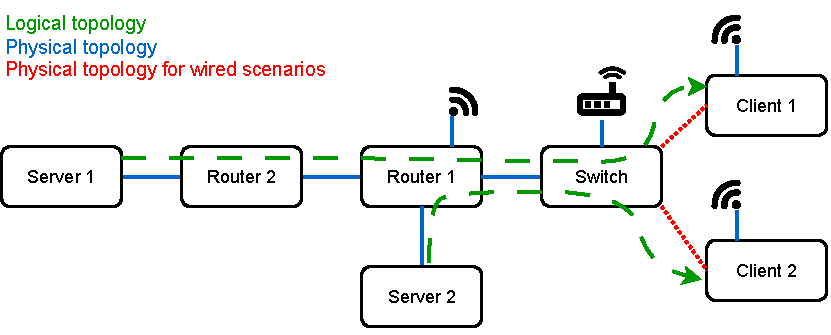
\includegraphics[height=0.28\textheight]{figures/topology-wireless.drawio-1.pdf}
};
\end{tikzpicture}


\begin{itemize}[<+->]
\item Server~2 \(\to\) Client~2: Always the same VoIP traffic
\item Server~1 \(\to\) Client~1:
\begin{itemize}
\item Three Reno flows
\item Three Cubic flows
\item Three BBR flows
\item One of each
\item The above, but also with VoIP
\end{itemize}
\end{itemize}
\end{frame}
\begin{frame}[label={sec:orgcb51d7c}]{Router settings}
\begin{tikzpicture}[remember picture, overlay]
\node[below left] at (current page.north east)
{
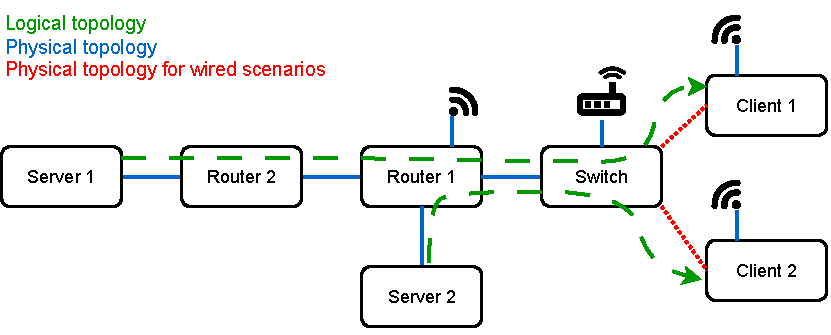
\includegraphics[height=0.28\textheight]{figures/topology-wireless.drawio-1.pdf}
};
\end{tikzpicture}

\begin{columns}
\begin{column}{.5\columnwidth}
\begin{block}{Buffer lengths at Router 1}
\begin{itemize}
\item 0.5 BDP
\item 1 BDP
\item 1.5 BDP
\item 2 BDP
\end{itemize}
\end{block}
\end{column}
\begin{column}{.5\columnwidth}
\begin{block}{Delay}
\begin{itemize}
\item 10ms
\item 50ms
\end{itemize}
\end{block}
\end{column}
\end{columns}
\end{frame}
\begin{frame}[label={sec:org58fe05d}]{Some fun numbers}
\begin{tikzpicture}[remember picture, overlay]
\node[below left] at (current page.north east)
{
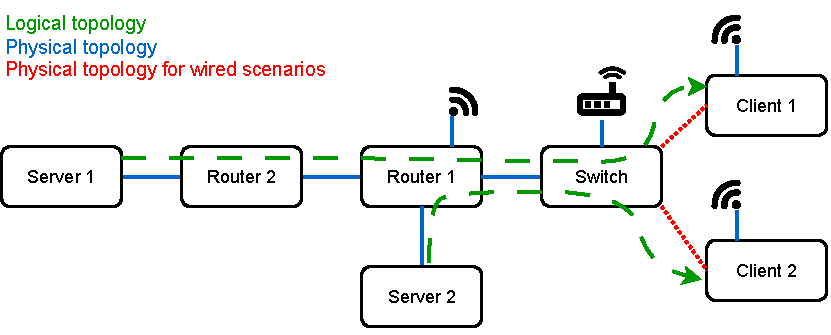
\includegraphics[height=0.28\textheight]{figures/topology-wireless.drawio-1.pdf}
};
\end{tikzpicture}


\begin{itemize}[<+->]
\item 64 different BDP + delay + capacity configurations
\item 192 total tests
\item 16 Hours of test time
\item >20 hours of TEACUP run time
\item \(\sim\)85 000 000 datapoints in total
\end{itemize}
\end{frame}
\begin{frame}[label={sec:org0ca37af}]{The correlation}
\begin{center}
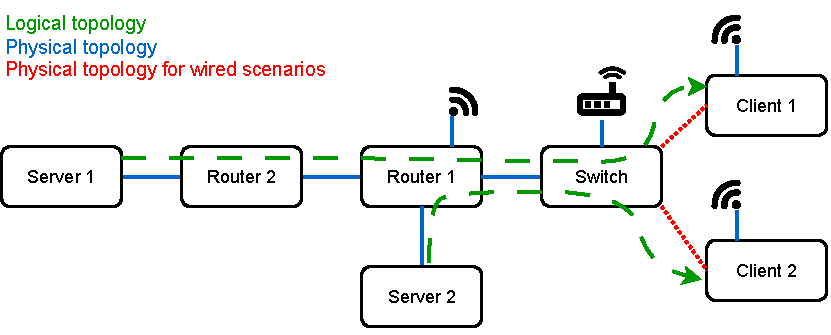
\includegraphics[width=.9\linewidth]{figures/topology-wireless.drawio-1.pdf}
\end{center}

See if the OWD of packets traveling towards Client 1 and Client 2 are correlated
\end{frame}
\begin{frame}[label={sec:orga6d0eeb}]{The correlation}
\begin{columns}
\begin{column}{.56\columnwidth}
\begin{figure}[htbp]
\centering
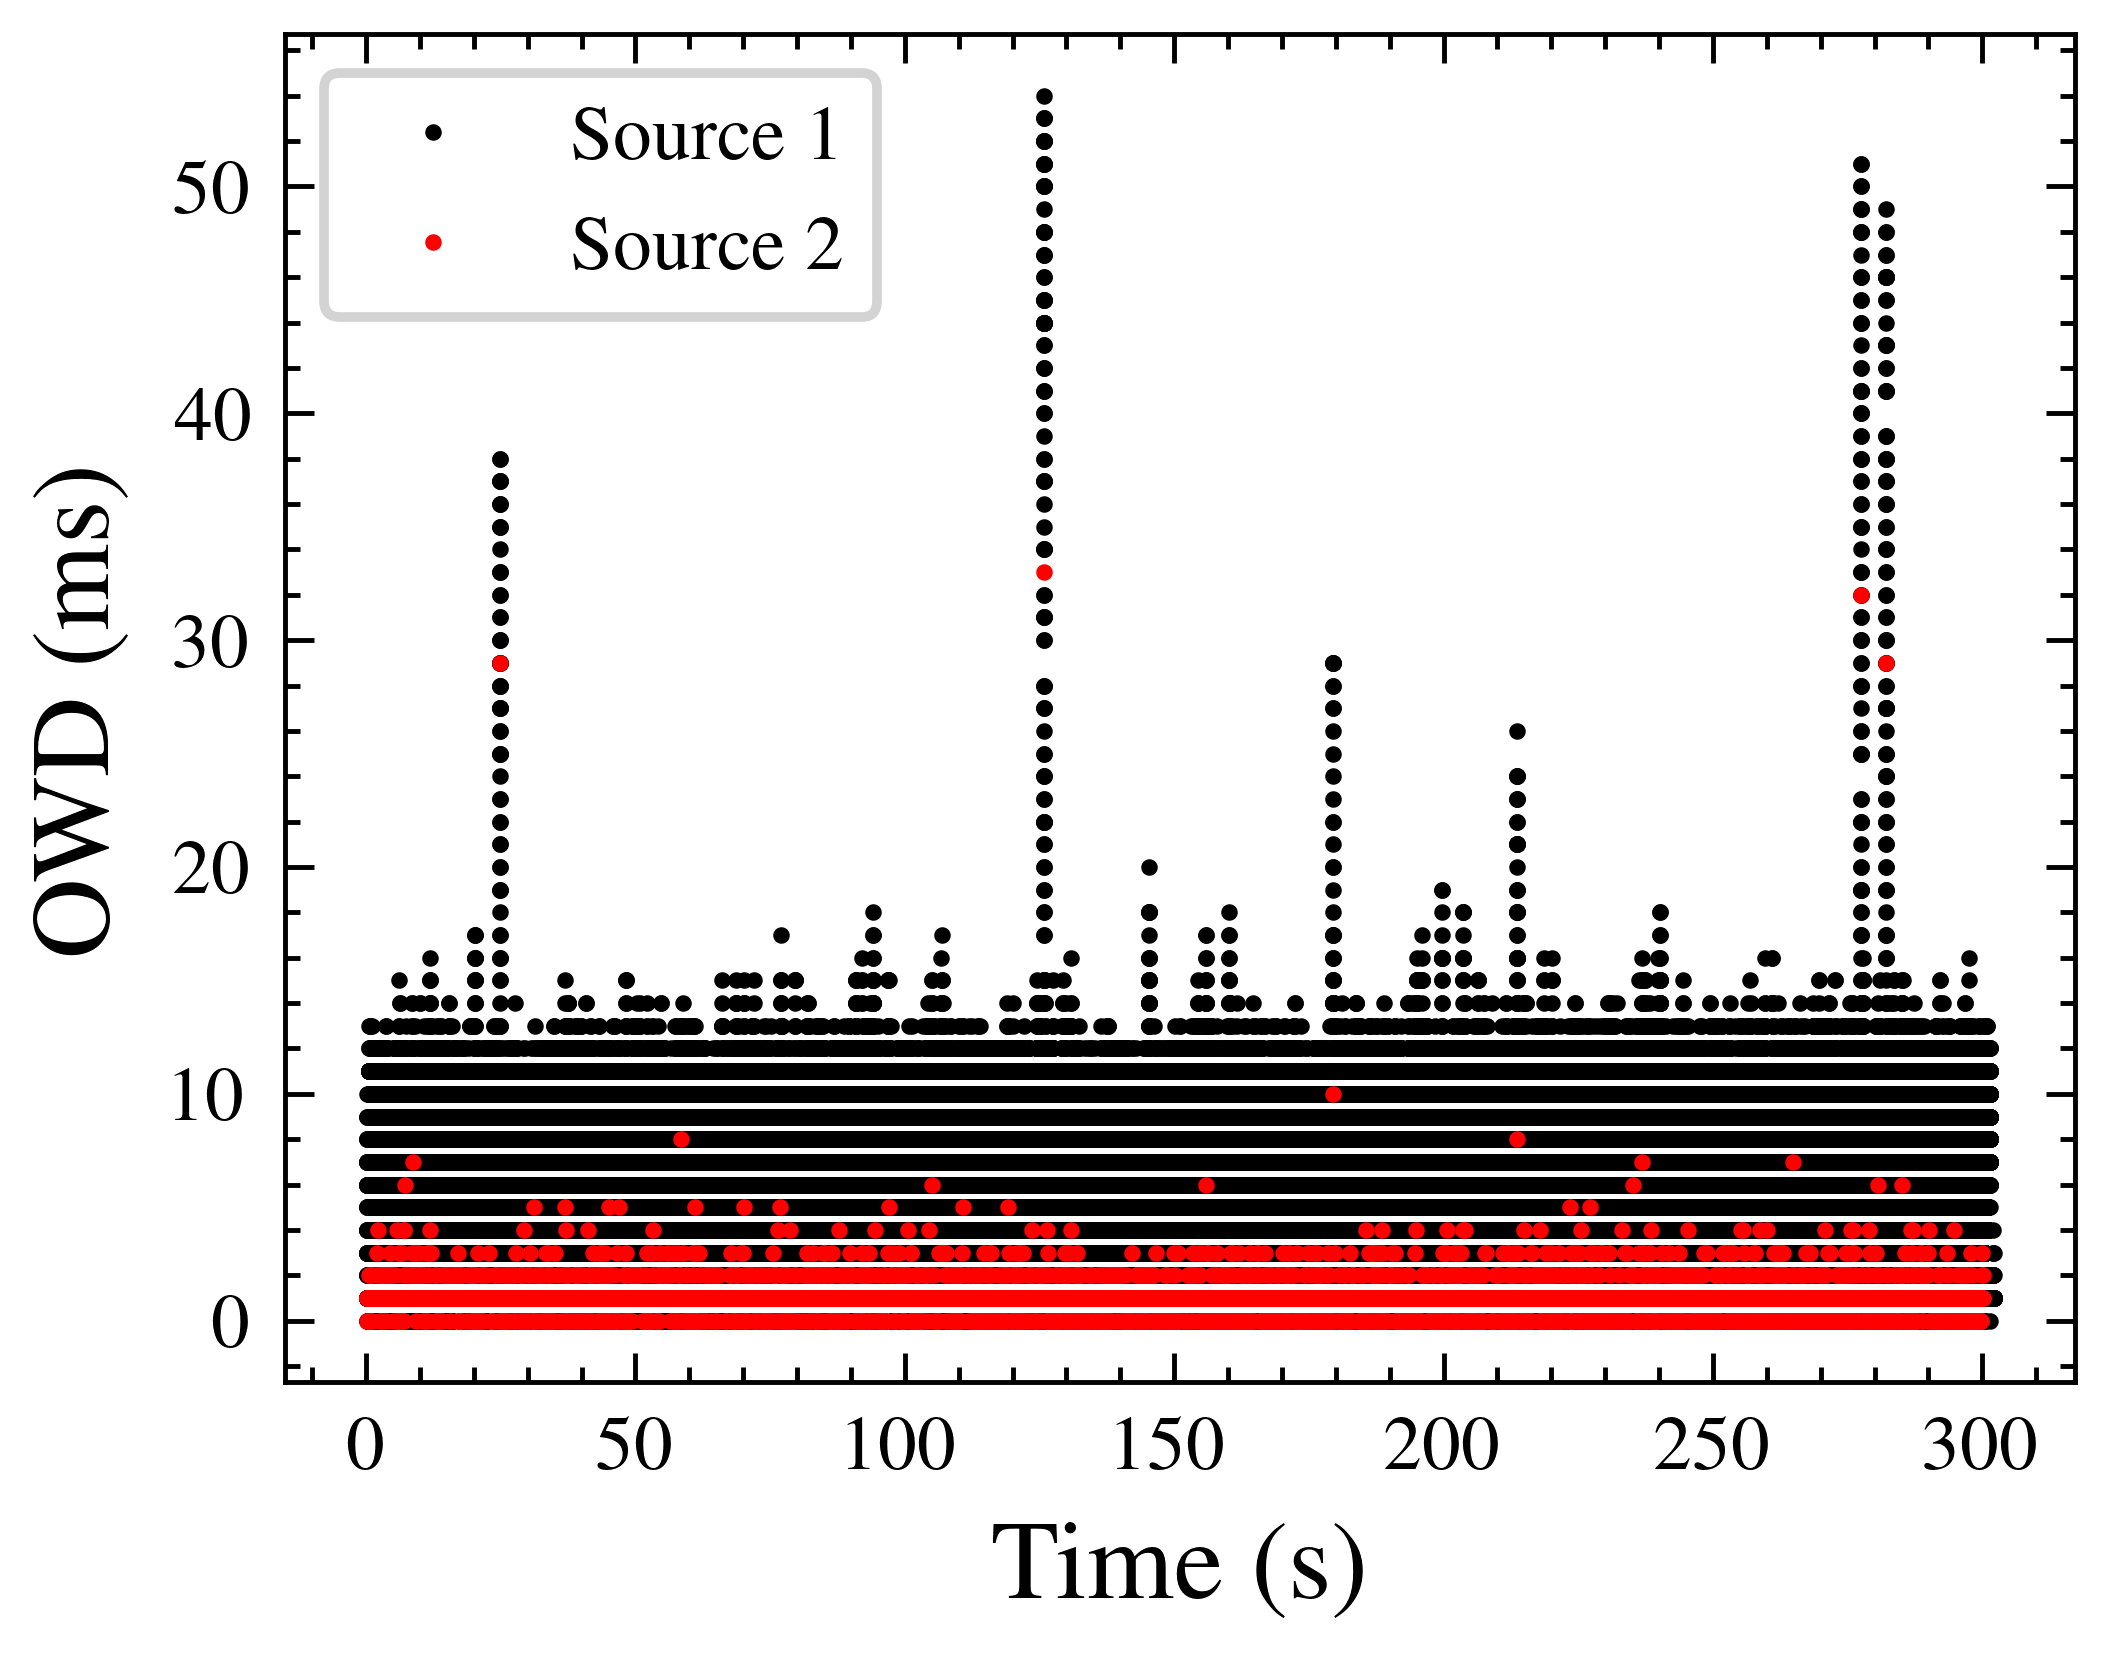
\includegraphics[width=.9\linewidth]{figures/presentation/owd-time-nocommon.png}
\caption{\label{fig:orgfc19fb7}No common bottleneck}
\end{figure}

\begin{itemize}[<3->]
\item Correlation: 0.20
\end{itemize}
\end{column}
\begin{column}{.56\columnwidth}
\pause
\begin{figure}[htbp]
\centering
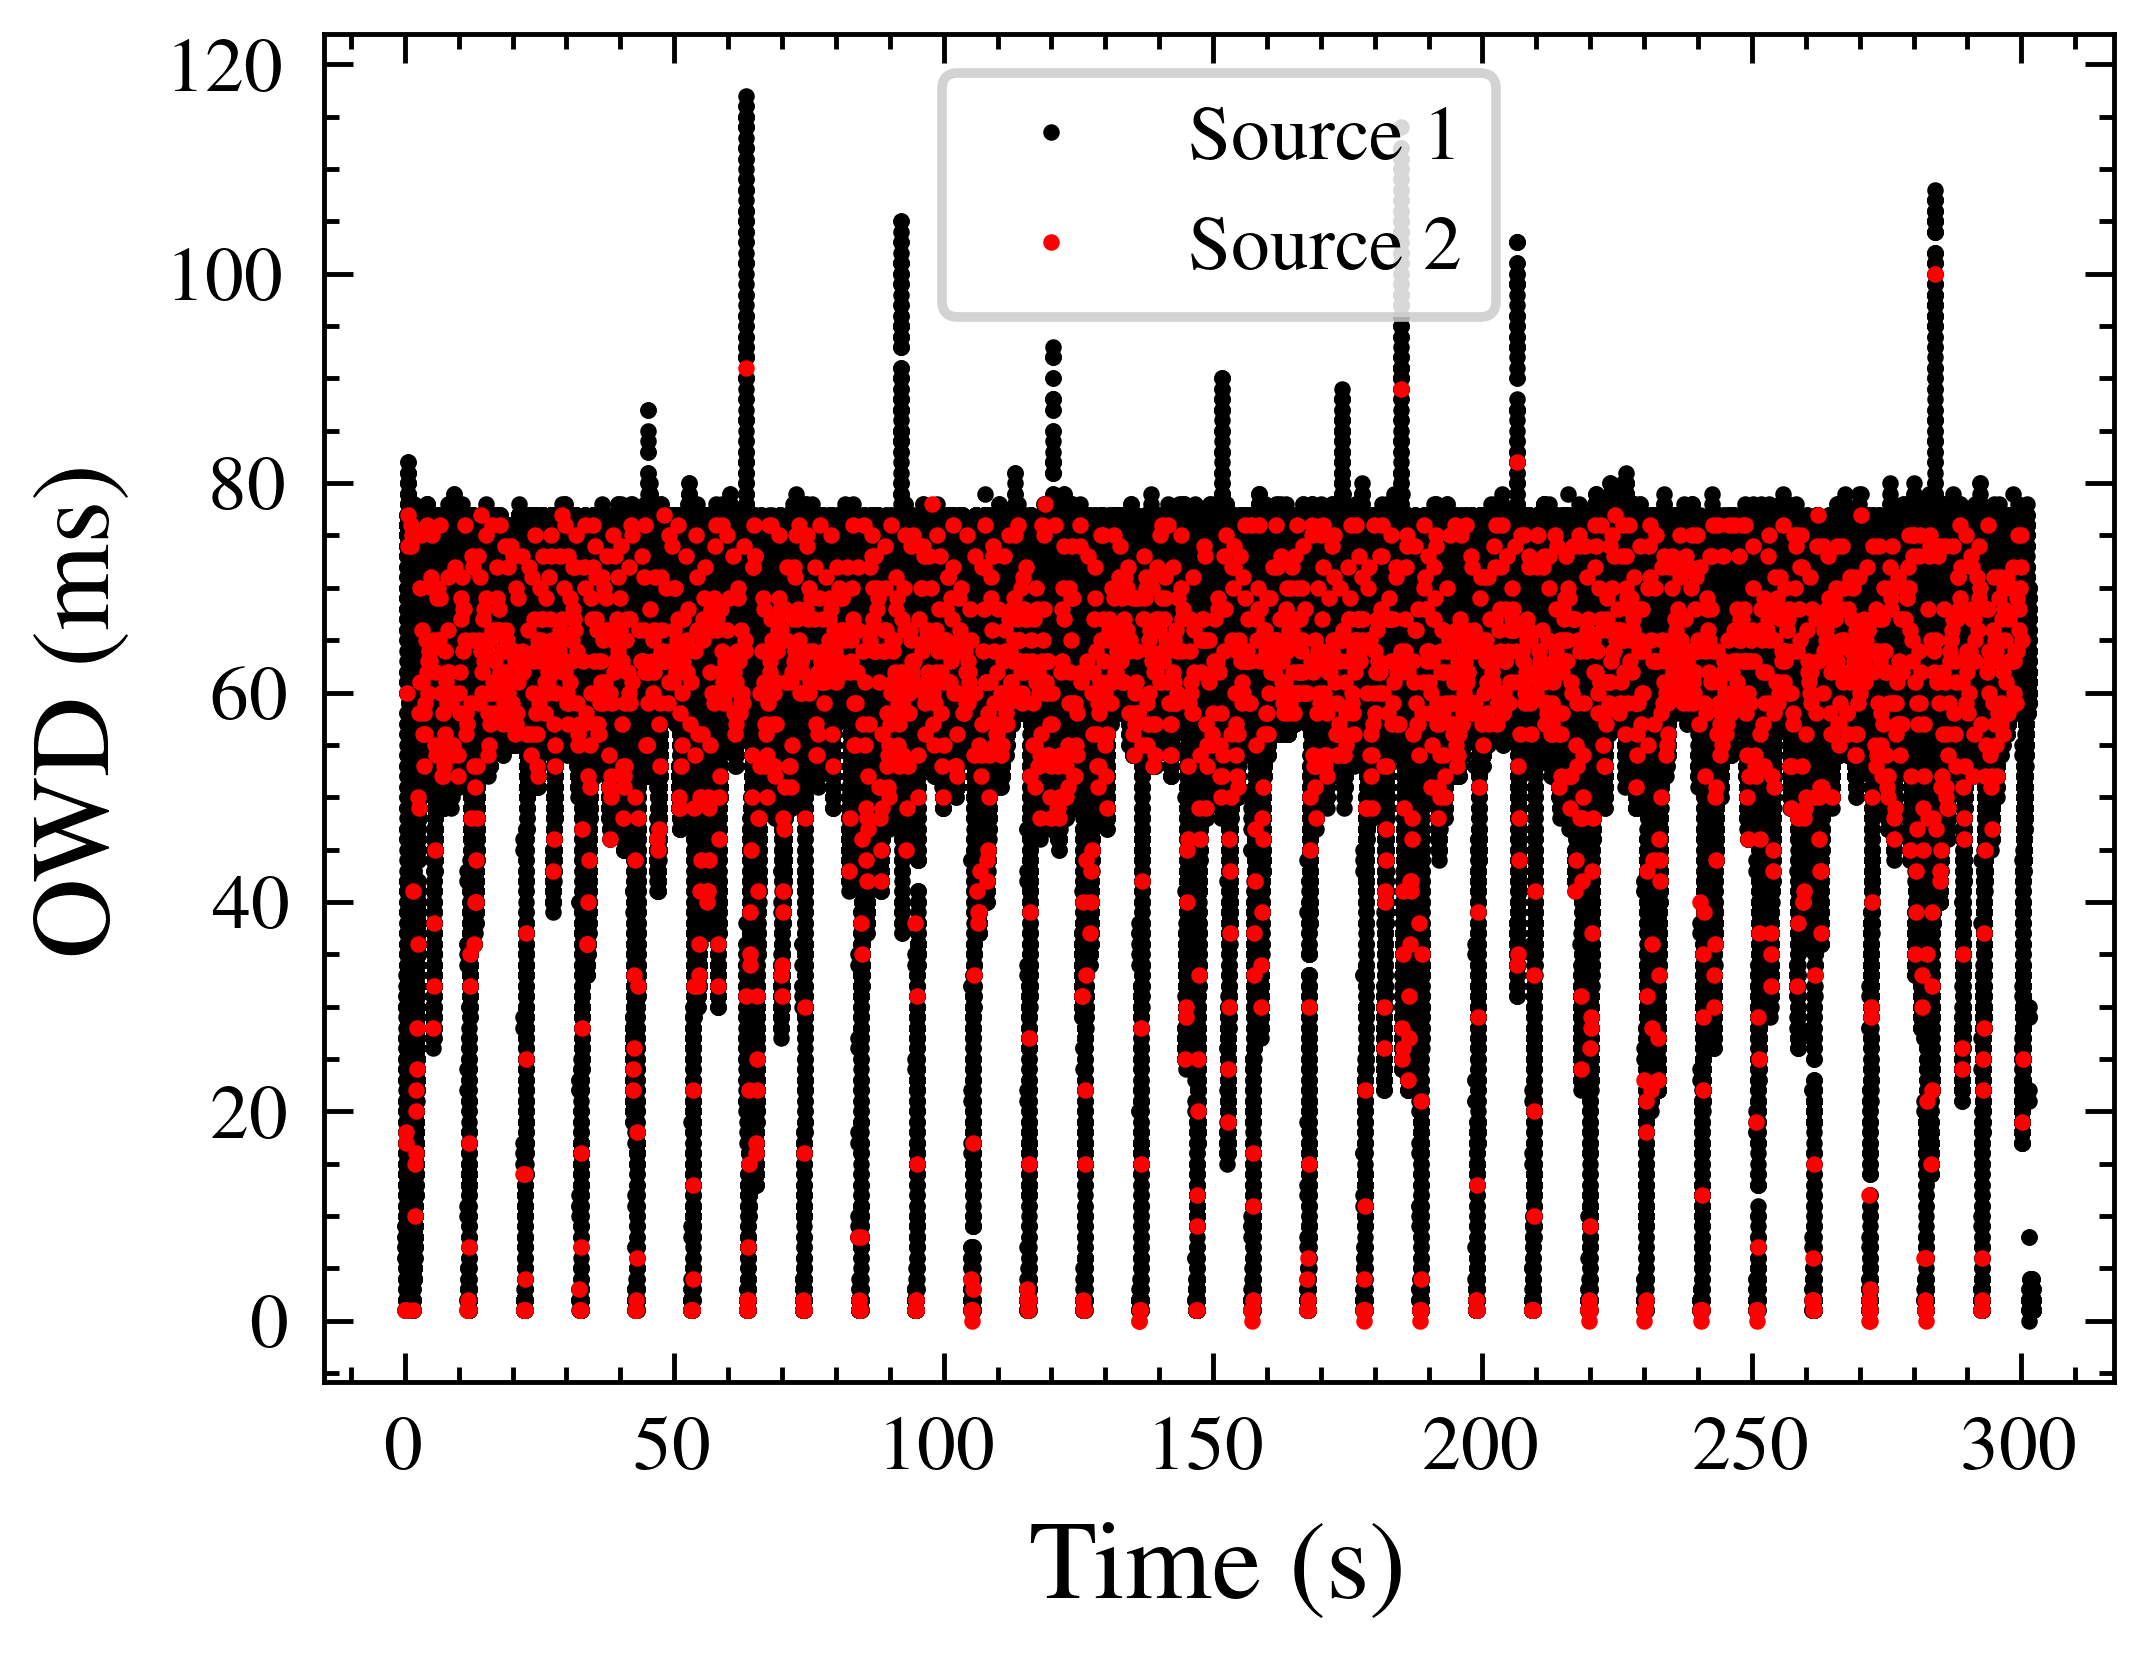
\includegraphics[width=.9\linewidth]{figures/presentation/owd-time-common.png}
\caption{\label{fig:orgf4f8970}Common bottleneck}
\end{figure}

\begin{itemize}[<3->]
\item Correlation: 0.93
\end{itemize}
\end{column}
\end{columns}
\end{frame}
\begin{frame}[label={sec:orgc68c5c5}]{CDF graph}
\begin{center}
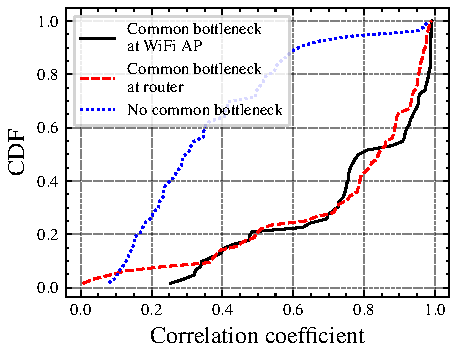
\includegraphics[width=.9\linewidth]{figures/results/all-over2-no-only-video.pdf}
\end{center}
\end{frame}
\begin{frame}[label={sec:org1501fd3}]{Traffic types}
\begin{tikzpicture}[remember picture, overlay]
\node[below left] at (current page.north east)
{
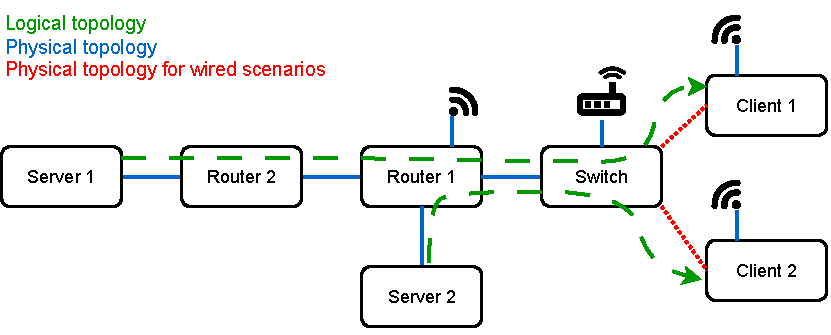
\includegraphics[height=0.28\textheight]{figures/topology-wireless.drawio-1.pdf}
};
\end{tikzpicture}


\begin{itemize}
\item Server~2 \(\to\) Client~2: Always the same VoIP traffic
\item Server~1 \(\to\) Client~1:
\begin{itemize}
\item Three Reno flows
\item Three Cubic flows
\item Three BBR flows
\item One of each
\item The above, but also with VoIP
\end{itemize}
\end{itemize}
\end{frame}
\begin{frame}[label={sec:org9e8bf03}]{Without VoIP}
\begin{center}
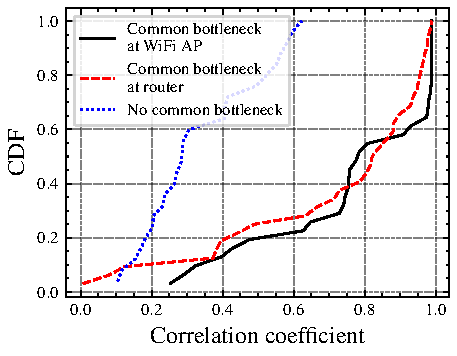
\includegraphics[width=.9\linewidth]{figures/results/all-over2-no-video.pdf}
\end{center}
\end{frame}
\begin{frame}[allowframebreaks,label=]{Correlation of CDF}
\begin{columns}
\begin{column}{.56\columnwidth}
\begin{figure}[htbp]
\centering
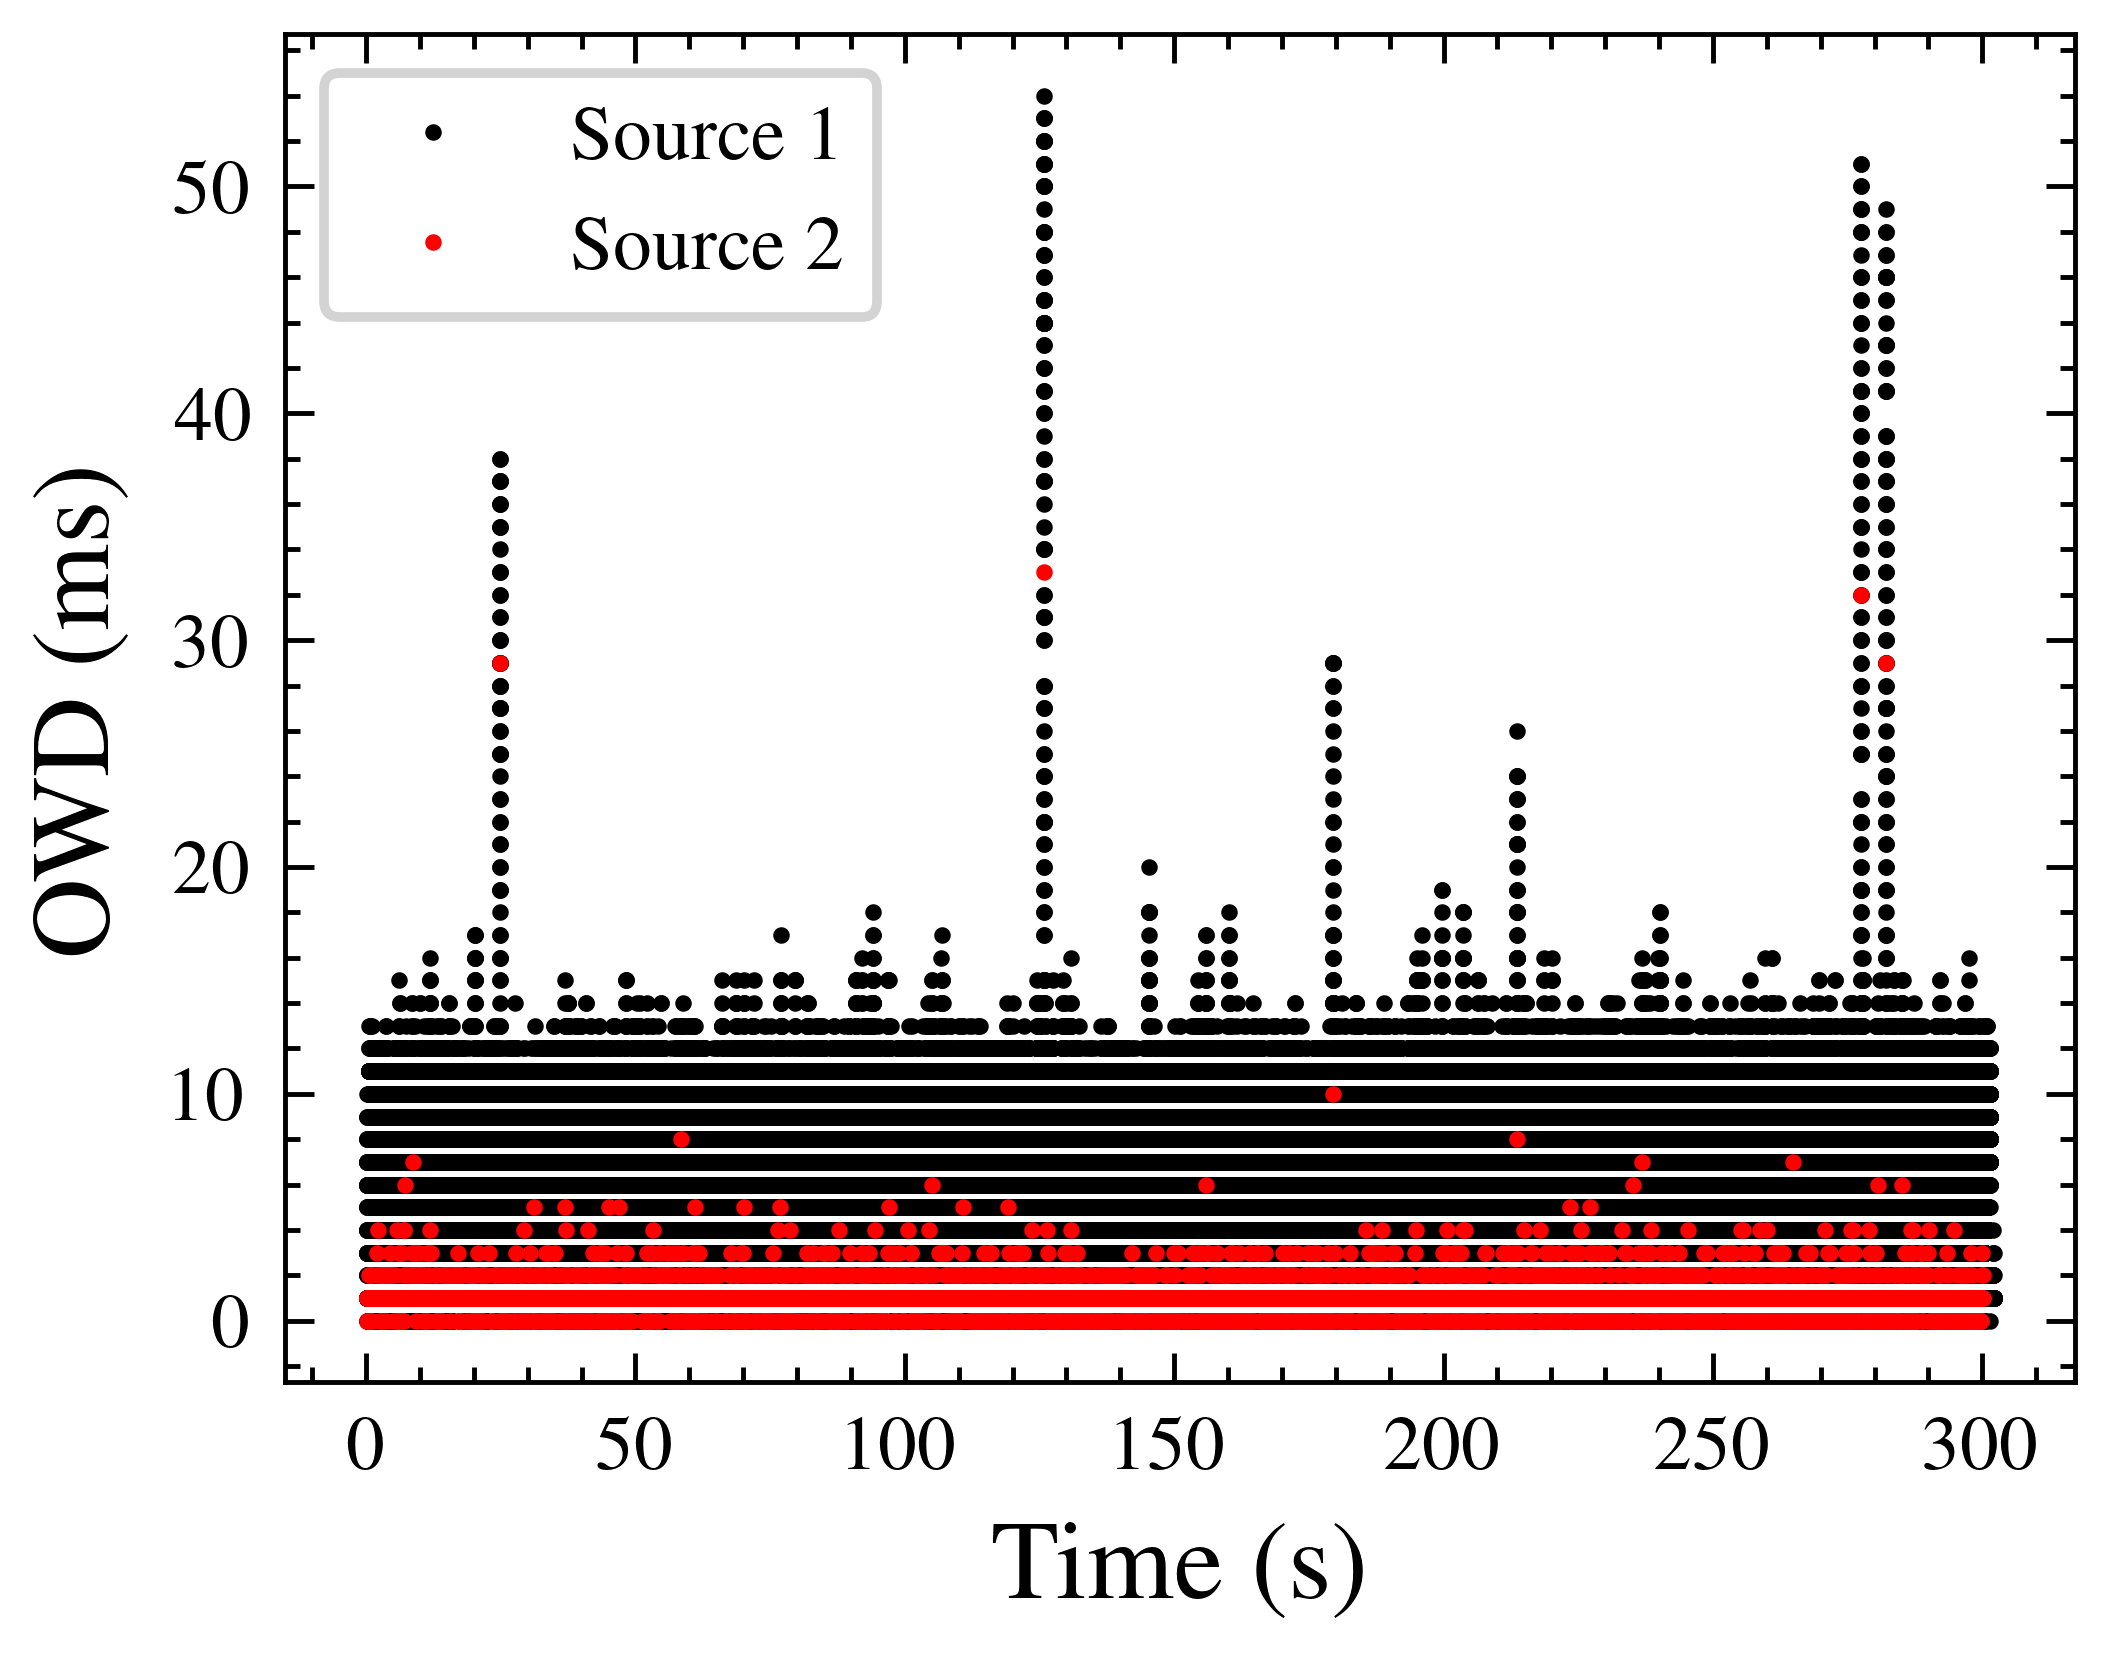
\includegraphics[width=.9\linewidth]{figures/presentation/owd-time-nocommon.png}
\caption{\label{fig:org40086b4}No common bottleneck}
\end{figure}

\begin{itemize}
\item Correlation: 0.20
\end{itemize}
\end{column}
\begin{column}{.56\columnwidth}
\begin{figure}[htbp]
\centering
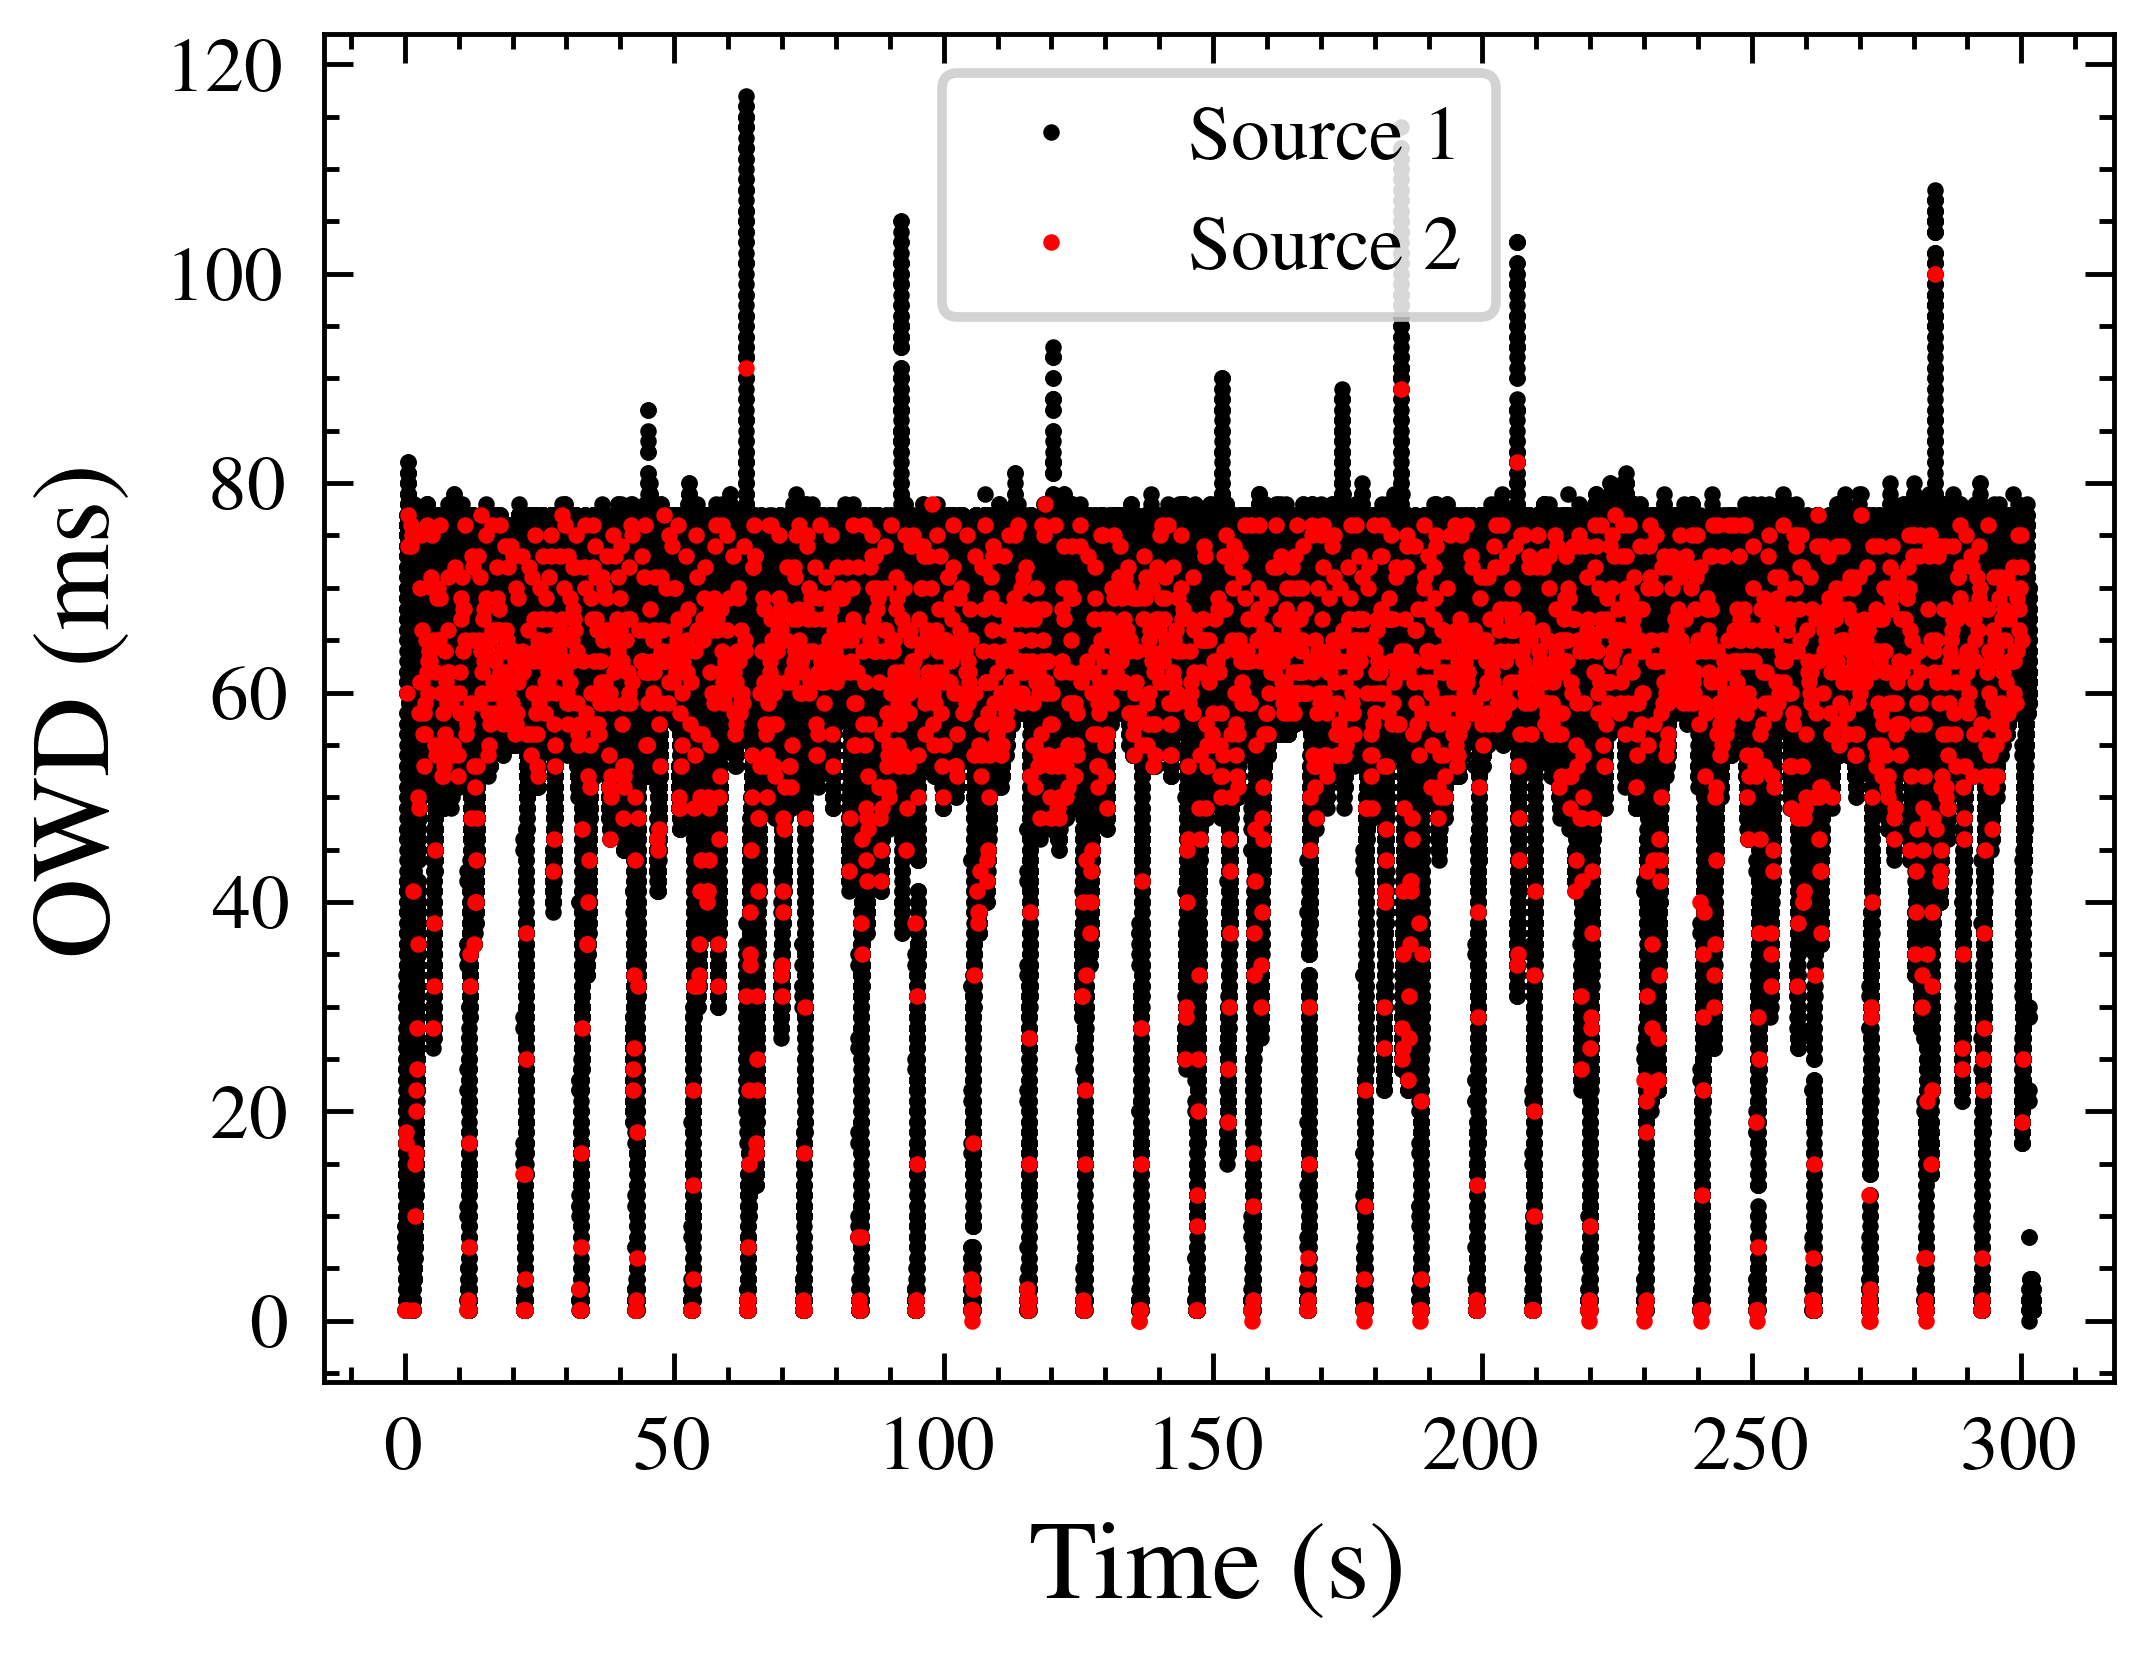
\includegraphics[width=.9\linewidth]{figures/presentation/owd-time-common.png}
\caption{\label{fig:orgaa82937}Common bottleneck}
\end{figure}

\begin{itemize}
\item Correlation: 0.93
\end{itemize}
\end{column}
\end{columns}
\framebreak
\begin{columns}
\begin{column}{.56\columnwidth}
\begin{figure}[htbp]
\centering
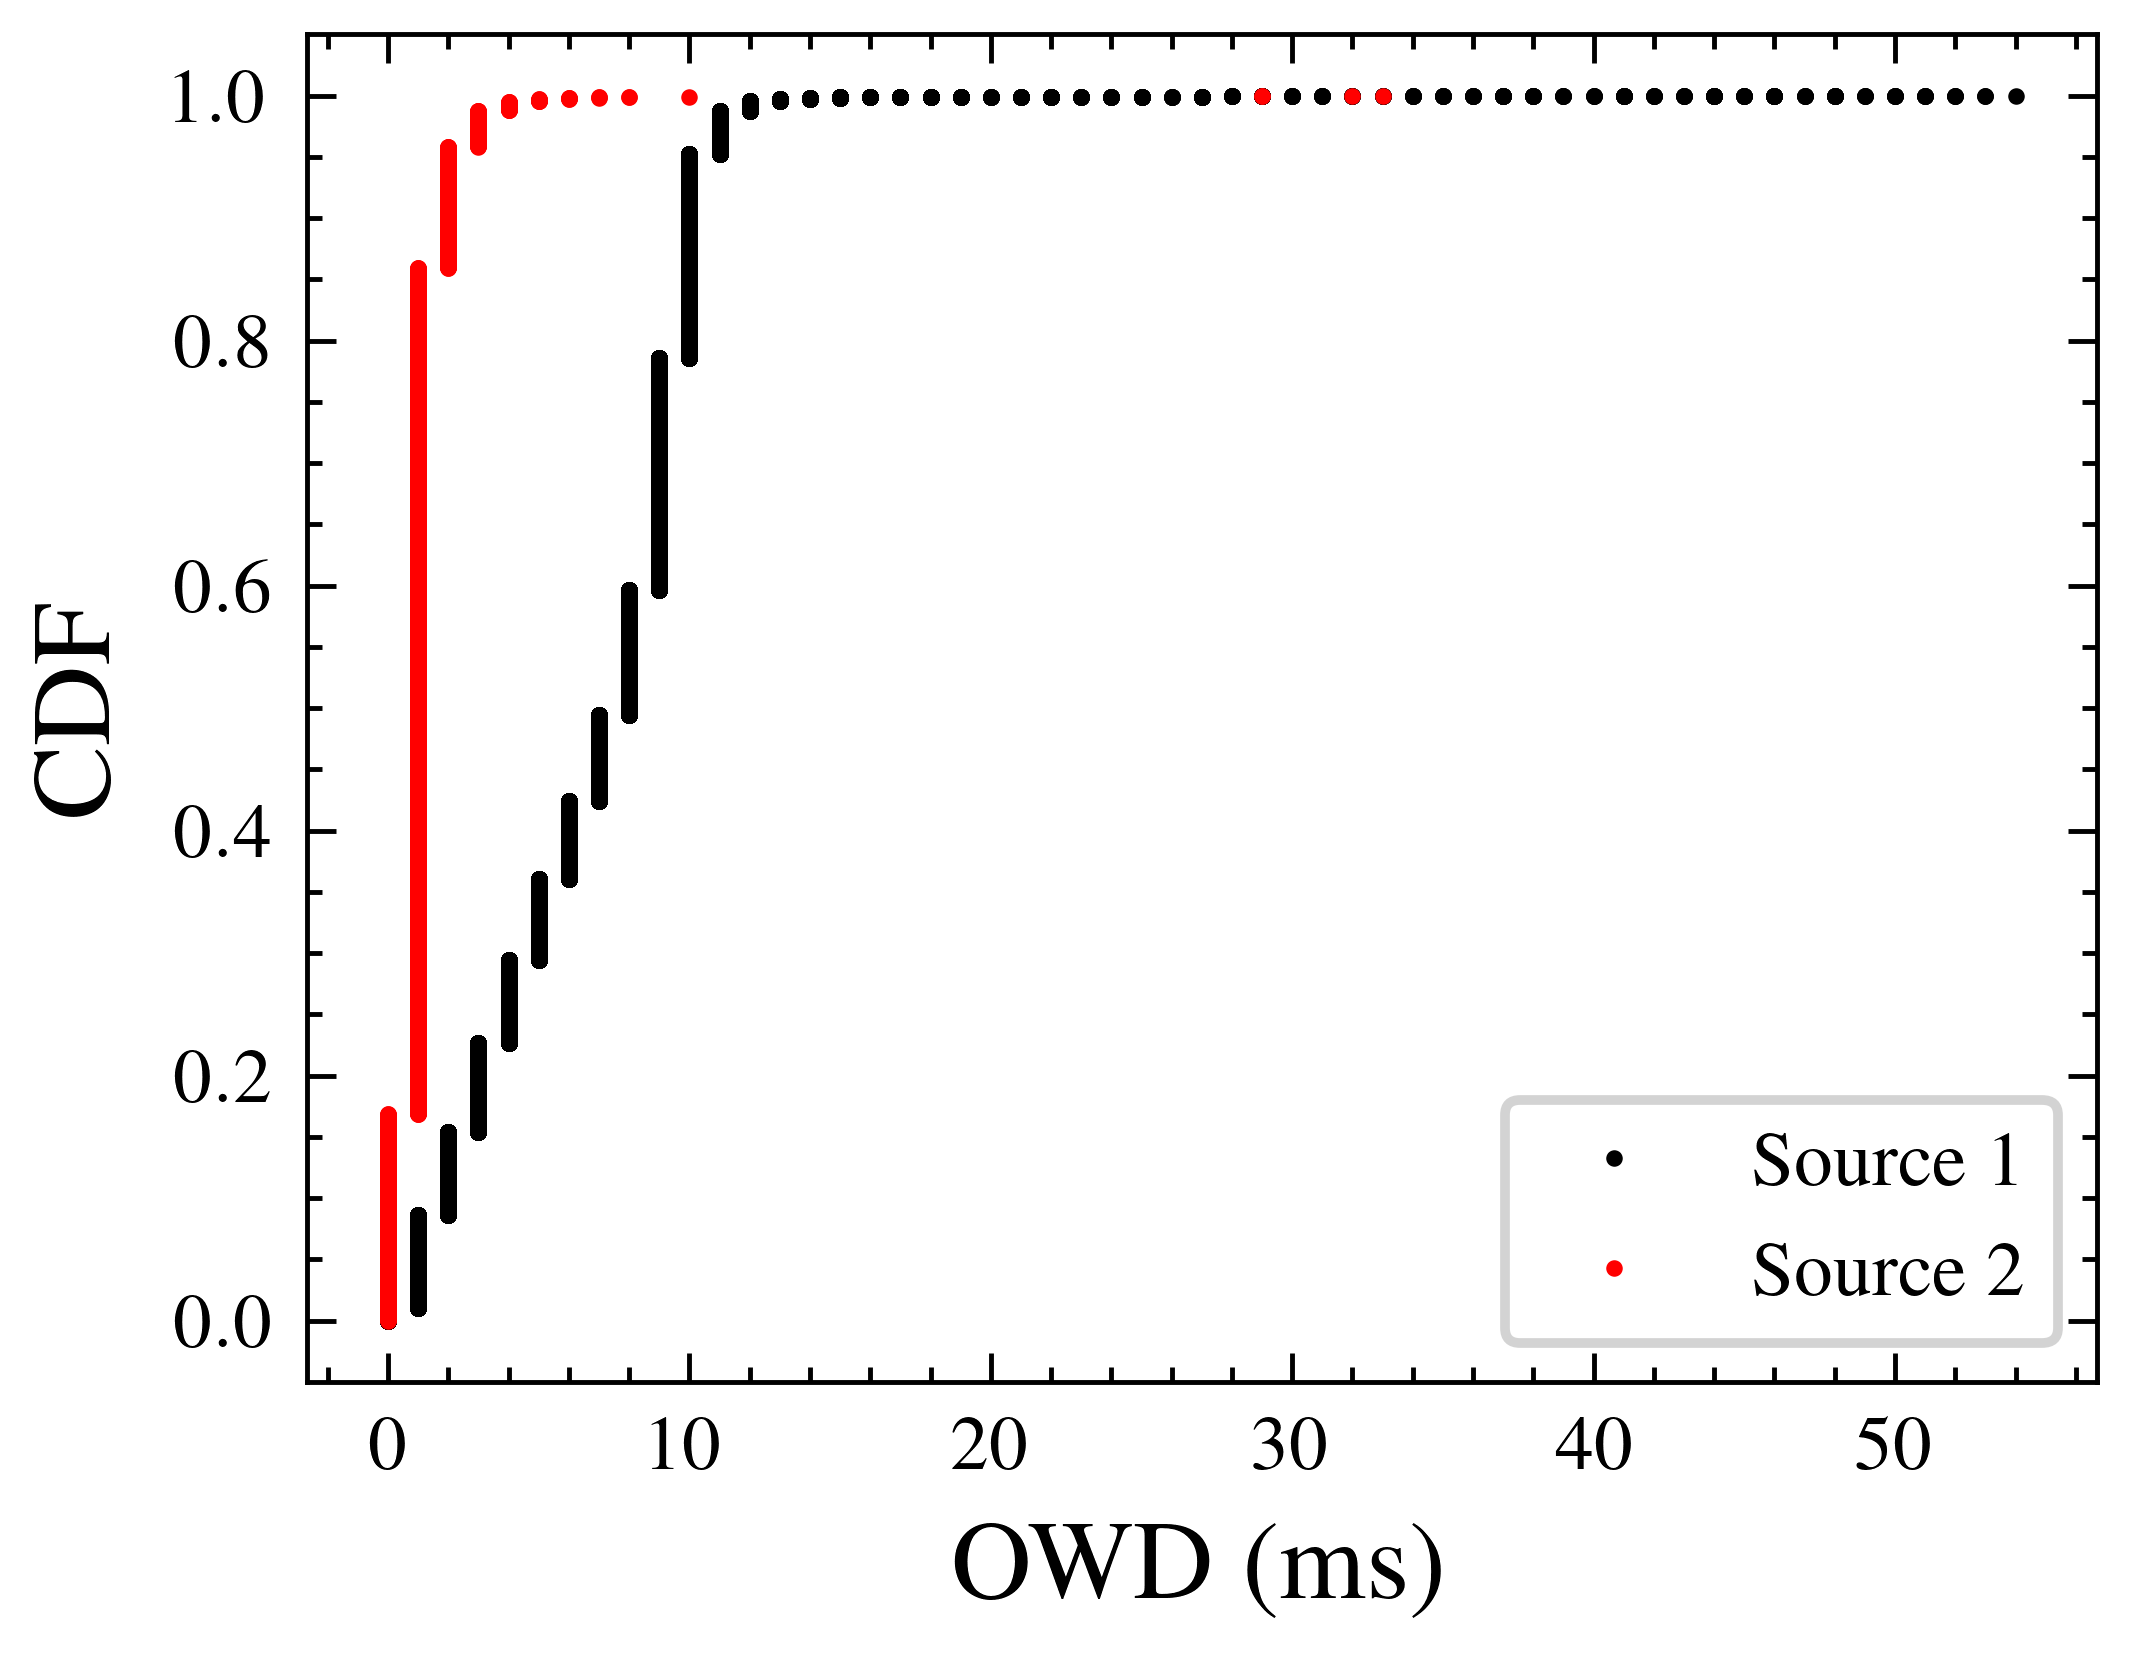
\includegraphics[width=.9\linewidth]{figures/presentation/correlation-owd-nocommon.png}
\caption{\label{fig:org98441fd}No common bottleneck}
\end{figure}

\begin{itemize}
\item Correlation: 0.4
\end{itemize}
\end{column}
\begin{column}{.56\columnwidth}
\begin{figure}[htbp]
\centering
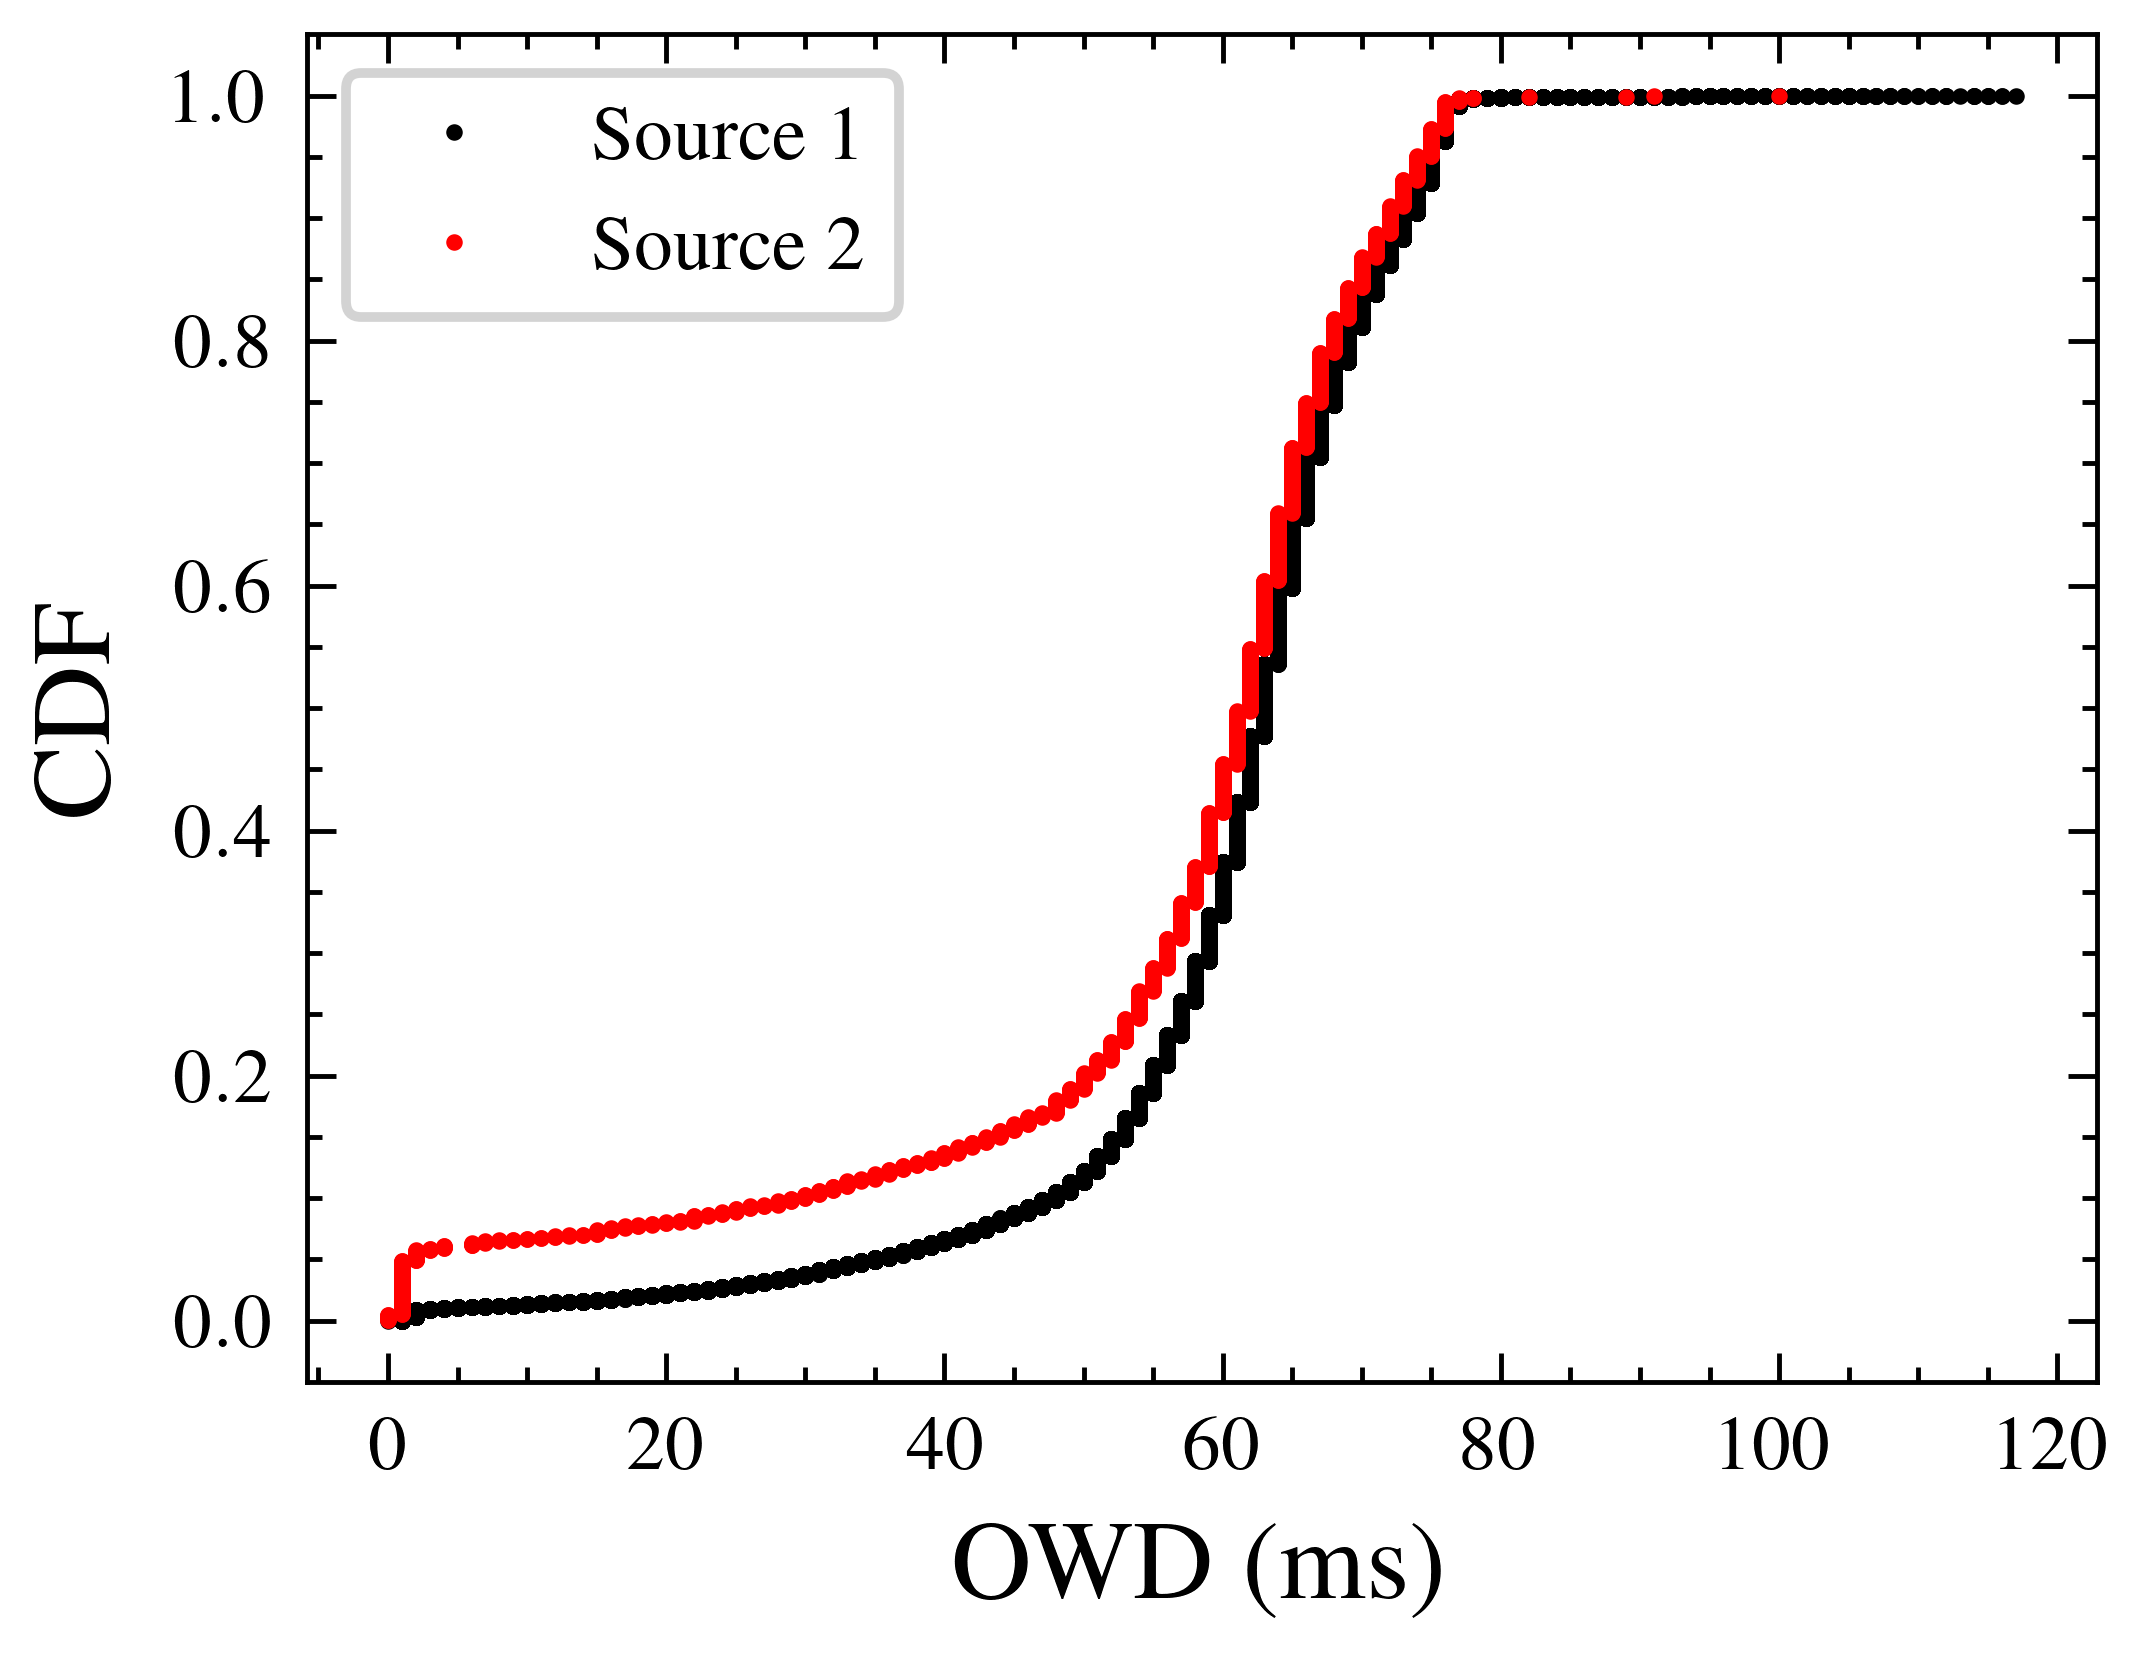
\includegraphics[width=.9\linewidth]{figures/presentation/correlation-owd-common.png}
\caption{\label{fig:org3d18c1c}Common bottleneck}
\end{figure}

\begin{itemize}
\item Correlation: 0.9967
\end{itemize}
\end{column}
\end{columns}
\begin{center}
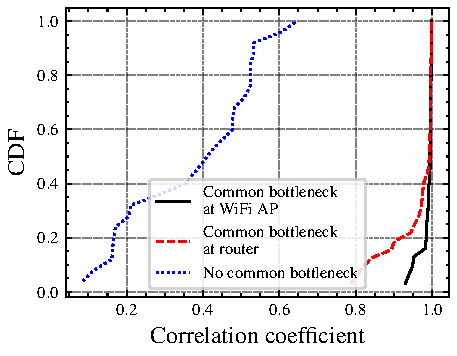
\includegraphics[width=.9\linewidth]{figures/double-cdf/double-cdf-all-over2-no-video.pdf}
\end{center}
\end{frame}
\end{document}
